\documentclass[11pt, letterpaper]{article}

\usepackage[margin=1in]{geometry}
\usepackage[T1]{fontenc}
\usepackage[utf8]{inputenc}
\usepackage{enumitem}
\usepackage{xcolor}
\usepackage{parskip}
\usepackage{booktabs}
\usepackage{tabularx}
\usepackage{tikz}
\usetikzlibrary{positioning, arrows.meta, shapes.geometric}

% Clean sans-serif font
\usepackage{helvet}
\renewcommand{\familydefault}{\sfdefault}

% Accent colors
\definecolor{accent}{RGB}{51, 65, 85}
\definecolor{tier1}{RGB}{22, 163, 74}
\definecolor{tier2}{RGB}{37, 99, 235}
\definecolor{tier3}{RGB}{147, 51, 234}
\definecolor{tier4}{RGB}{234, 88, 12}

\begin{document}

\begin{center}
{\Large \textbf{The Chronological Process of Digitizing Construction}}\\[0.5em]
{\color{accent}\small From Design Model to Project Closeout}\\[0.3em]
{\small Matt Pappas | Kiewit Data \& Analytics | \today}
\end{center}

\vspace{1.5em}

\section*{Executive Summary}

Construction project execution follows an immutable sequence. Quantities must exist before costs can be estimated. Costs must be estimated before schedules can be built. Schedules must exist before procurement can be timed. Procurement and schedules must align before work can be planned. Work plans must exist before safety and quality requirements can be attached. And only then can execution begin, monitored against the plan.

Any digitization strategy that ignores this chronology will fail. Systems built out of sequence require rework as upstream capabilities mature. This paper defines the eight-stage lifecycle and maps each stage to the digital capabilities required to support it.

\vspace{1em}

\begin{center}
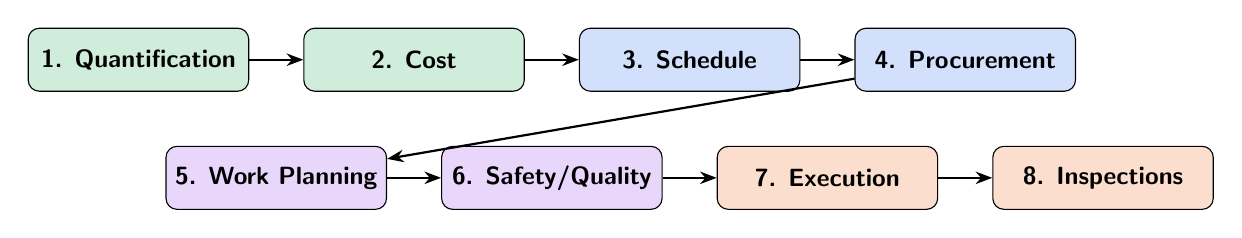
\begin{tikzpicture}[
    node distance=0.3cm,
    stage/.style={draw, rounded corners=4pt, minimum width=2.8cm, minimum height=0.8cm, align=center, font=\small\bfseries},
    arrow/.style={-{Stealth[length=6pt]}, thick}
]
    \node[stage, fill=tier1!20] (q) at (0,0) {1. Quantification};
    \node[stage, fill=tier1!20] (c) at (3.5,0) {2. Cost};
    \node[stage, fill=tier2!20] (s) at (7,0) {3. Schedule};
    \node[stage, fill=tier2!20] (p) at (10.5,0) {4. Procurement};
    
    \node[stage, fill=tier3!20] (w) at (1.75,-1.5) {5. Work Planning};
    \node[stage, fill=tier3!20] (sq) at (5.25,-1.5) {6. Safety/Quality};
    \node[stage, fill=tier4!20] (e) at (8.75,-1.5) {7. Execution};
    \node[stage, fill=tier4!20] (i) at (12.25,-1.5) {8. Inspections};
    
    \draw[arrow] (q) -- (c);
    \draw[arrow] (c) -- (s);
    \draw[arrow] (s) -- (p);
    \draw[arrow] (p) -- (w);
    \draw[arrow] (w) -- (sq);
    \draw[arrow] (sq) -- (e);
    \draw[arrow] (e) -- (i);
\end{tikzpicture}
\end{center}

\vspace{1.5em}

\section*{Stage 1: Quantification}

\textbf{Definition:} Extract and normalize the physical scope of work from engineering deliverables---design models (BIM/CAD), drawings (2D), and specifications.

\textbf{What happens here:}
\begin{itemize}
    \item Engineered equipment is identified and cataloged (pumps, vessels, structural steel, electrical panels, etc.)
    \item Design specifications are parsed for material requirements, tolerances, and installation constraints
    \item Quantities are extracted from 3D models (cubic yards of concrete, linear feet of pipe, tons of steel)
    \item Quantities are normalized to a master reference data structure (account codes) that the rest of the organization understands
    \item Material ontology mapping connects design nomenclature to procurement and estimating nomenclature
\end{itemize}

\textbf{Why this is foundational:}

Every downstream process depends on knowing \textit{what} is being built and \textit{how much}. An estimate without quantities is a guess. A schedule without quantities cannot determine durations. Procurement without quantities cannot size orders. Work planning without quantities cannot scope work packages.

\textbf{Digital capabilities required:}
\begin{itemize}
    \item Design model ingestion pipeline (BIM/CAD to data lake)
    \item PDF/drawing quantity extraction (for 2D deliverables)
    \item Vision models for automated takeoff
    \item Material ontology and master data management
    \item Quantity normalization and standardization engine
\end{itemize}

\textbf{Related KIP Use Cases:} C4 (Estimate Takeoff), C10 (Project Takeoff Feed to Plan \& Procurement), C12 (Project Quantity Overrun Tracking), C14 (Model Visualization and Usage Standards), E2 (Construction and Procurement Model Exports), P2 (Takeoff)

\vspace{1em}

\hrule

\vspace{1em}

\section*{Stage 2: Cost}

\textbf{Definition:} Establish a terminal quantity baseline and apply unit costs to produce a project estimate.

\textbf{What happens here:}
\begin{itemize}
    \item Terminal quantities are locked as the basis for the estimate (the ``quantity freeze'')
    \item Unit costs are applied---labor rates, material prices, equipment costs, subcontractor pricing
    \item Estimate conformance aligns quantities to standard account codes and business line structures
    \item Roll-ups aggregate detail-level costs into summary categories (by discipline, by area, by phase)
    \item Risk analysis identifies quantities with high likelihood of overrun based on historical data
    \item The estimate becomes the cost baseline against which project performance is measured
\end{itemize}

\textbf{Why sequence matters:}

The estimate is only as accurate as the quantities it is built on. If quantities change after the estimate is locked, the estimate must be reworked. If the quantity extraction process is immature, the estimate will require constant revision as the design matures.

\textbf{Digital capabilities required:}
\begin{itemize}
    \item Estimating system integration (InEight Estimate)
    \item Automated estimate conformance (account code mapping, roll-ups, splits)
    \item Parametric estimating for early-stage estimates
    \item Historical cost database with unit rate benchmarking
    \item Quantity-to-estimate traceability (what quantities drive which cost lines)
\end{itemize}

\textbf{Related KIP Use Cases:} C5 (Estimate Creation), C6 (Estimate Conformance), E4 (Estimate Creation), P3 (Estimating)

\vspace{1em}

\hrule

\vspace{1em}

\section*{Stage 3: Schedule}

\textbf{Definition:} Build a time-phased plan that sequences work activities based on quantities, logic relationships, and resource constraints.

\textbf{What happens here:}
\begin{itemize}
    \item Work breakdown structure (WBS) is defined---the hierarchy of deliverables and activities
    \item Activities are created and linked to quantities (e.g., ``Install 500 LF of 6'' pipe'' drives a duration)
    \item Logic relationships (predecessors/successors) are established based on construction sequence
    \item Durations are calculated from quantities, productivity rates, and crew sizes
    \item Resources (labor, equipment) are loaded against activities
    \item Critical path is identified---the sequence of activities that determines project duration
    \item Milestones are set for engineering, procurement, and construction phases
\end{itemize}

\textbf{Why sequence matters:}

Schedules built without accurate quantities produce unreliable durations. A schedule that assumes 1,000 LF of pipe when the actual quantity is 1,500 LF will be wrong by 50\%. If quantities are still being refined when the schedule is built, the schedule will require constant rework.

\textbf{Digital capabilities required:}
\begin{itemize}
    \item Scheduling system integration (Primavera P6, InEight Schedule)
    \item Automated schedule generation from estimate/quantity data
    \item Historical productivity database (hours per unit by activity type)
    \item Resource leveling and optimization
    \item Critical path analysis and what-if scenario modeling
    \item Integrated master schedule across construction, engineering, and procurement
\end{itemize}

\textbf{Related KIP Use Cases:} C7 (Project Schedule Creation), C8 (Project Risk Creation and Monitoring), E7 (Schedule Creation), P4 (Schedule)

\vspace{1em}

\hrule

\vspace{1em}

\section*{Stage 4: Procurement}

\textbf{Definition:} Source materials, equipment, and subcontractor services timed to the construction schedule.

\textbf{What happens here:}
\begin{itemize}
    \item Procurement packages are scoped based on quantities and specifications
    \item Vendor qualification and selection---matching suppliers to package requirements
    \item RFQs are issued and quotes are compared (supplier quote comparison)
    \item Purchase orders and subcontracts are executed
    \item Procurement schedule is built---lead times, fabrication windows, delivery dates
    \item Material delivery is coordinated with construction need dates
    \item Vendor performance is tracked (on-time delivery, quality, cost conformance)
\end{itemize}

\textbf{Why sequence matters:}

Procurement cannot be scoped without knowing what to buy (quantities) and when it is needed (schedule). Ordering too early ties up capital and storage space. Ordering too late causes construction delays. The procurement schedule must be derived from the construction schedule, not created independently.

\textbf{Digital capabilities required:}
\begin{itemize}
    \item Procurement system integration
    \item Supplier quote comparison and analysis (Source360)
    \item Procurement schedule generation from construction schedule
    \item Vendor qualification and performance tracking
    \item Material tracking and visibility
    \item Lead time management and expediting alerts
\end{itemize}

\textbf{Related KIP Use Cases:} P4 (Schedule), P5 (Vendor Selection), P6 (Vendor Status), P7 (Contract Management), P8 (Vendor Selection - Performance), P9 (Material Visibility)

\vspace{1em}

\hrule

\vspace{1em}

\section*{Stage 5: Work Planning}

\textbf{Definition:} Decompose the schedule into executable work packages that can be assigned to crews.

\textbf{What happens here:}
\begin{itemize}
    \item Work packages are created---discrete scopes of work with defined boundaries
    \item Each work package includes: scope (what), quantities (how much), schedule (when), resources (who/what equipment)
    \item Constraints are identified---prerequisite work, material availability, equipment availability, access
    \item Short interval plans (SIPs) break work packages into daily/weekly executable tasks
    \item Crew assignments match labor resources to work package requirements
    \item Work package release gates ensure all prerequisites are met before work begins
\end{itemize}

\textbf{Why sequence matters:}

Work packages cannot be created without quantities (scope), estimates (resource requirements), schedules (timing), and procurement status (material availability). A work package released before materials arrive causes crew idle time. A work package released before predecessor work is complete causes rework.

\textbf{Digital capabilities required:}
\begin{itemize}
    \item Work package generation from schedule and quantity data
    \item Short interval planning automation
    \item Constraint management and release gate tracking
    \item Crew assignment and labor balancing
    \item Work package status tracking and completion reporting
\end{itemize}

\textbf{Related KIP Use Cases:} C13 (Work Package Creation), C19 (Short Interval Planning Creation), C21 (Auto progress schedule from component claiming)

\vspace{1em}

\hrule

\vspace{1em}

\section*{Stage 6: Safety, Quality, and Compliance}

\textbf{Definition:} Attach safety requirements, quality hold points, and compliance documentation to work packages before execution begins.

\textbf{What happens here:}
\begin{itemize}
    \item Safety hazards are identified for each work package (fall protection, confined space, electrical, excavation)
    \item Job Hazard Analyses (JHAs) are created or referenced from historical templates
    \item Required PPE, permits, and safety procedures are specified
    \item Quality hold points are defined---inspection requirements before proceeding to next phase
    \item Inspection test plans (ITPs) are attached to work packages
    \item Compliance forms are pre-populated based on work type and regulatory requirements
    \item Environmental requirements are documented (dust control, stormwater, waste disposal)
\end{itemize}

\textbf{Why sequence matters:}

Safety and quality requirements must be attached \textit{before} work begins, not discovered during execution. If work packages are released without safety plans, crews proceed without adequate protection. If quality hold points are not defined, inspection opportunities are missed and rework results.

\textbf{Digital capabilities required:}
\begin{itemize}
    \item Automated compliance form generation based on work type
    \item Safety hazard prediction from historical incident data
    \item Quality checklist generation based on work package scope
    \item Inspection test plan management
    \item Permit tracking and status visibility
\end{itemize}

\textbf{Related KIP Use Cases:} C15 (Safety and quality management), C16 (Safety management), C17 (Compliance Form Creation), C18 (Completion Form Creation)

\vspace{1em}

\hrule

\vspace{1em}

\section*{Stage 7: Execution Monitoring}

\textbf{Definition:} Track progress against the plan, capture actuals, and identify variances in real time.

\textbf{What happens here:}
\begin{itemize}
    \item Quantities installed are reported daily (units completed, percent complete)
    \item Labor hours are captured against work packages and activities
    \item Schedule progress is updated---actual start/finish dates, remaining duration
    \item Earned value is calculated---comparing planned progress to actual progress to actual cost
    \item Variances are identified---schedule slippage, cost overruns, productivity issues
    \item Change orders are processed---scope changes, claims, schedule impacts
    \item Forecasts are updated---estimate at completion, projected finish date
\end{itemize}

\textbf{Why sequence matters:}

Execution monitoring compares actuals to the plan. If the plan (quantities, estimates, schedule, work packages) is unreliable, monitoring produces meaningless variances. Garbage in, garbage out. The quality of execution monitoring is directly proportional to the quality of the upstream planning.

\textbf{Digital capabilities required:}
\begin{itemize}
    \item Mobile quantity claiming from the field
    \item Automated schedule progress updates from component claiming
    \item Real-time cost reporting and earned value calculation
    \item Variance analysis and exception alerting
    \item Change order management and impact analysis
    \item Forecast modeling and scenario planning
\end{itemize}

\textbf{Related KIP Use Cases:} C9 (Change order management), C11 (Resource management), C20 (Quantity Claiming), C21 (Auto progress schedule), C22 (Project Billings), C23 (Project Month End Status Report)

\vspace{1em}

\hrule

\vspace{1em}

\section*{Stage 8: Inspections and Closeout}

\textbf{Definition:} Verify work meets specifications, document completion, and close out work packages.

\textbf{What happens here:}
\begin{itemize}
    \item Quality inspections are performed at defined hold points
    \item Non-conformances are documented and tracked to resolution
    \item Punch lists capture remaining deficiencies before turnover
    \item As-built documentation is compiled---what was actually installed vs. design
    \item Test and commissioning procedures verify systems operate as designed
    \item Turnover packages are assembled for owner acceptance
    \item Lessons learned are captured for future projects
\end{itemize}

\textbf{Why sequence matters:}

Inspections verify that execution matched the plan. If the plan was poorly defined (vague specifications, missing quality requirements), inspections cannot determine conformance. If execution monitoring was inadequate, inspection findings are surprises rather than confirmations.

\textbf{Digital capabilities required:}
\begin{itemize}
    \item Digital inspection checklists with photo documentation
    \item Non-conformance tracking and resolution workflow
    \item Punch list management
    \item As-built documentation compilation
    \item Turnover package assembly and tracking
    \item Lessons learned database
\end{itemize}

\textbf{Related KIP Use Cases:} C15 (Safety and quality management), C18 (Completion Form Creation)

\vspace{1.5em}

\section*{The Rework Risk of Building Out of Sequence}

The eight stages form a dependency chain. Each stage consumes outputs from the previous stage and produces inputs for the next. When digitization efforts skip stages or build downstream before upstream is mature, three failure modes emerge:

\textbf{1. Data Mismatch}

If the estimating system is digitized before quantity extraction is standardized, estimates are built on inconsistent quantity data. When quantity extraction matures and produces different (more accurate) numbers, every estimate must be rebuilt.

\textbf{2. Integration Rework}

If the scheduling system is digitized independently from the estimating system, the integration between them must be built twice---once with the immature interface, and again when the upstream system changes.

\textbf{3. User Distrust}

If execution monitoring is digitized before the plan is reliable, field teams see meaningless variances and lose trust in the system. Regaining trust after a failed rollout is harder than building trust the first time.

\vspace{1em}

\begin{center}
\textit{The cost of building out of sequence is not just rework---it is compounding rework.\\Each downstream system that depends on an immature upstream system inherits its instability.}
\end{center}

\vspace{1.5em}

\section*{Recommended Digitization Sequence}

Based on the chronological dependencies, the recommended digitization sequence is:

\begin{enumerate}
    \item \textbf{Quantification (Months 1--12):} Design model ingestion, quantity extraction, material ontology, master data management. This is the foundation. Do not proceed until quantities flow reliably.
    
    \item \textbf{Cost (Months 6--18):} Estimating system integration, automated conformance, quantity-to-estimate traceability. Begin after Quantification demonstrates stable output.
    
    \item \textbf{Schedule (Months 12--24):} Schedule generation from estimates, productivity database, integrated master schedule. Begin after Cost produces reliable estimates.
    
    \item \textbf{Procurement (Months 12--24):} Procurement schedule derivation, vendor selection, material tracking. Can run parallel with Schedule since both consume Cost outputs.
    
    \item \textbf{Work Planning (Months 18--30):} Work package generation, short interval planning, constraint management. Begin after Schedule and Procurement are integrated.
    
    \item \textbf{Safety/Quality (Months 18--30):} Compliance forms, hazard prediction, inspection test plans. Can run parallel with Work Planning.
    
    \item \textbf{Execution Monitoring (Months 24--36):} Quantity claiming, progress updates, earned value, change orders. Begin after Work Planning produces reliable packages.
    
    \item \textbf{Inspections (Months 30--42):} Digital inspections, punch lists, turnover packages. Begin after Execution Monitoring demonstrates reliable actuals capture.
\end{enumerate}

\vspace{0.5em}

Total timeline: 36--42 months for full lifecycle digitization.

\vspace{0.5em}

\textit{Attempting to compress this timeline by running stages in parallel before their upstream dependencies are stable will extend the timeline through rework, not shorten it.}

\end{document}

